% Generated 2021-08-25 18:02:25 +0530
\subsection{QIF} \label{sec:QIF}


This section provides the semantic information for the \block{QIFDocumentWrapper} model.

\begin{figure}[ht]
  \centering
    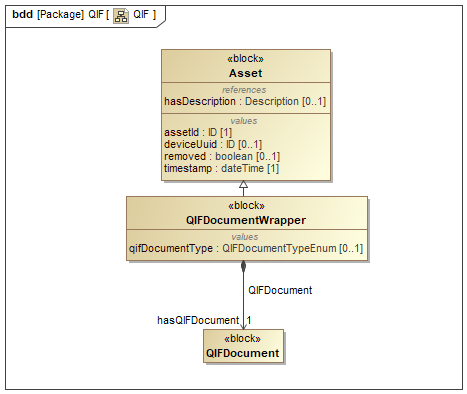
\includegraphics[width=1.0\textwidth]{figures/QIFDocumentWrapper.png}
  \caption{QIFDocumentWrapper Diagram}
  \label{fig:QIFDocumentWrapper Diagram}
\end{figure}

\FloatBarrier


Note: See \sect{QIFDocumentWrapper Schema Diagrams} for XML schema.



\subsubsection{QIFDocument}
\label{sec:QIFDocument}



The QIF Document as given by the QIF standard.



\subsubsection{QIFDocumentWrapper}
\label{sec:QIFDocumentWrapper}



An \gls{MTConnect Asset} carrying the Quality Information Framework (QIF) Document.


\paragraph{Attributes of QIFDocumentWrapper}\mbox{}
\label{sec:Attributes of QIFDocumentWrapper}

\tbl{Attributes of QIFDocumentWrapper} lists the attributes of \texttt{QIFDocumentWrapper}.

\begin{table}[ht]
\centering 
  \caption{Attributes of QIFDocumentWrapper}
  \label{table:Attributes of QIFDocumentWrapper}
\tabulinesep=3pt
\begin{tabu} to 6in {|l|l|l|} \everyrow{\hline}
\hline
\rowfont\bfseries {Attribute} & {Type} & {Multiplicity} \\
\tabucline[1.5pt]{}

\property{qifDocumentType}[QIFDocumentWrapper] & \texttt{QIFDocumentTypeEnum} & 0..1 \\
\end{tabu}
\end{table}
\FloatBarrier

Descriptions for attributes of \block{QIFDocumentWrapper}:

\begin{itemize}

\item \property{qifDocumentType}[QIFDocumentWrapper] \newline The contained QIF Document type as defined in the QIF Standard.

\texttt{QIFDocumentTypeEnum} Enumeration:

\begin{itemize}
\item \texttt{MEASUREMENT\textunderscore RESOURCE} \newline  
\item \texttt{PLAN} \newline  
\item \texttt{PRODUCT} \newline  
\item \texttt{RESULTS} \newline  
\item \texttt{RULES} \newline  
\item \texttt{STATISTICS} \newline  
\end{itemize}

\end{itemize}


\paragraph{Elements of QIFDocumentWrapper}\mbox{}
\label{sec:Elements of QIFDocumentWrapper}

\tbl{Elements of QIFDocumentWrapper} lists the elements of \texttt{QIFDocumentWrapper}.

\begin{table}[ht]
\centering 
  \caption{Elements of QIFDocumentWrapper}
  \label{table:Elements of QIFDocumentWrapper}
\tabulinesep=3pt
\begin{tabu} to 6in {|l|l|} \everyrow{\hline}
\hline
\rowfont\bfseries {Element} & {Multiplicity} \\
\tabucline[1.5pt]{}
\texttt{QIFDocument} & 1 \\
\end{tabu}
\end{table}
\FloatBarrier


Descriptions for elements of \block{QIFDocumentWrapper}:

\begin{itemize}

\item \block{QIFDocument} \newline The QIF Document as given by the QIF standard.
\end{itemize}


